\documentclass[]{article}
\usepackage{amssymb}
\usepackage{amstext}
\usepackage{amsmath}
\usepackage{amsthm}
\usepackage{graphicx} 
\usepackage{hyperref}

\newtheorem*{theorem}{Theorem}
\newtheorem*{definition}{Definition}
\newtheorem*{claim}{Claim}

%opening
\title{Neural Networks Can Approximate Continuous Functions}
\author{Paul Dubois}
\date{}

\begin{document}

\maketitle

\begin{abstract}
	A clean Tex version of the proof seen during the lectures that neural networks with ReLU activation can approximate continuous functions.
\end{abstract}

\section{Statement}
\begin{definition}
	$\mathcal{C}\left( \left[ a,b \right] \right)$ is the set of real continuous functions on $\left[ a,b \right]$.
\end{definition}
\begin{definition}
	$\mathcal{P}\left( n,l \right)$ is the set of rectangle 1D-1D perceptrons with $l$ hidden layers and $n$ neurons in each hidden layer.
\end{definition}

\begin{theorem}[Particular case of the universal approximation theorem\footnote{See \url{https://en.wikipedia.org/wiki/Universal_approximation_theorem} for details.}]
	$$\forall f \in \mathcal{C}(\left[ a,b \right]), \ \forall \varepsilon > 0, \ \exists N \in \mathbb{N} \text{ and } p \in \mathcal{P}(N,1) \text{ s.t. } \|p-f\|_\infty < \varepsilon$$
	Where $\|g\|_\infty$ is infinity norm of $g$ on $\left[ a,b \right]$; i.e. $\|g\|_\infty = \max_{x \in \left[ a,b \right]}(|g(x)|)$.
\end{theorem}


\section{Idea}
The idea of the proof is to split the interval $\left[ a,b \right]$ in sub intervals such that $f$ has variation less than $\varepsilon$ in the sub-intervals.
Then, choose the weights of the neural network to interpolate linearly $f$ et the beginning and end of the sub-intervals.
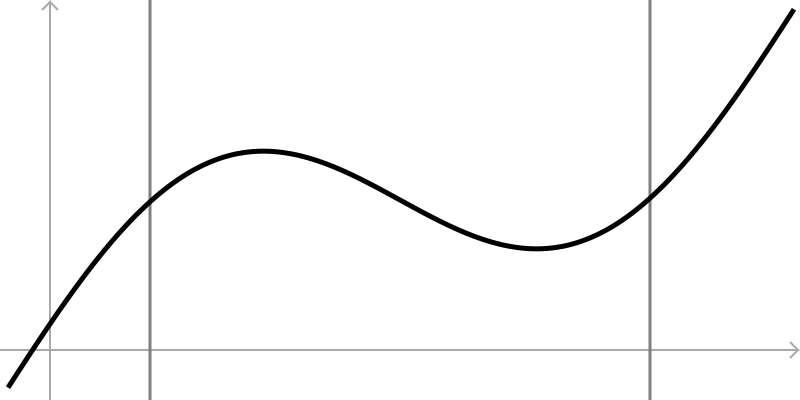
\includegraphics[width=\linewidth]{plot}

\section{Proof}
Let $\varepsilon >0$ and $f \in \mathcal{C}(\left[ a,b \right])$ with $a,b \in \mathbb{R}$, we want $N \in \mathbb{N}$ and $p \in \mathcal{P}(N,1)$ such that $\|p-f\|_\infty < \varepsilon$.

\paragraph{ReLU Network}
If $p \in \mathcal{P}(N,1)$, then 
$$p(x) = \xi + \sum_{k=0}^{N-1} \gamma_k (\alpha_k x + \beta_k)_+$$
where $(x)_+$ is $\text{ReLU}(x)$.

All we need to do is to find the right coefficients $\xi, \alpha_k, \beta_k, \gamma_k (0 \leq k < N)$ such that $|f(x)-p(x)| < \varepsilon \quad (\forall x \in \left[ a,b \right])$.

\paragraph{Uniform Continuity}
Since $f$ is continuous on a compact set, so $f$ is uniformly continuous.
Thus, $\forall x_1,x_2 \in \left[ a,b \right]$, $\exists \delta>0$ such that 
$$|x_1-x_2| < \delta \implies |f(x_1) - f(x_2)| < \varepsilon.$$

\paragraph{Sub-intervals}
Let $c_0 = a$ and $c_{i+1} = c_i + \delta$. Let $N \in \mathbb{N}$ be such that $c_N \geq b$ and redefine $c_N = b$.

\paragraph{Coefficients}
Take:
\begin{itemize}
	\item $\alpha_k = 1 \quad (0 \leq k < N)$
	\item $\beta_k = -c_k \quad (0 \leq k < N)$
	\item $\tilde{\gamma_k} = \frac{f(c_{k+1})-f(c_k)}{c_{k+1}-c_k} \quad (0 \leq k < N)$
	\item $\gamma_0 = \tilde{\gamma0}$
	\item $\gamma_k = \tilde{\gamma_{k+1}} - \tilde{\gamma_k}  \quad (0 < k < N)$
	\item $\xi = f(a)$
\end{itemize}
Thus, $$p(x) = \xi + \sum_{k=0}^{N-1} \gamma_k (\alpha_k x + \beta_k)_+$$
becomes $$p(x) = f(a) + \sum_{k=0}^{N-1} \gamma_k (x - c_k)_+.$$

\paragraph{Intermediate Result}
\begin{claim}[`The network interpolates linearly from $c_n$ to $c_{n+1}$']
	If $x \in \left[ c_n, c_{n+1} \right]$, then $p(x) = f(c_n) + \tilde{\gamma_n}(x-c_n)$.
\end{claim}
\begin{proof}
	\textbf{Case $k=0$:}\newline
	Let $x \in \left[ c_0, c_1 \right]$, then:
	$$p(x) = f(a) + \sum_{k=0}^{N-1} \gamma_k (x - c_k)_+$$
	since $x \leq c_1$, $(x - c_k)_+ = 0 \quad \forall k>0$, and $(x - c_k)_+ = x - c_k$: 
	$$p(x) = f(a) + \gamma_0 (x - c_0)$$
	as $\tilde{\gamma_0} =\gamma_0$ and $a = c_0$, we finally have $p(x) = f(a) + \tilde{\gamma_0}(x - c_0)$, as expected.
	
	\textbf{Recursion:}\newline
	\begin{itemize}
		\item Suppose that if $x \in \left[ c_n, c_{n+1} \right]$, then $p(x) = f(c_n) + \tilde{\gamma_n}(x-c_n)$.
		\item We want to show that if $x \in \left[ c_{n+1}, c_{n+2} \right]$, then $p(x) = f(c_{n+1}) + \tilde{\gamma_{n+1}}(x-c_{n+1})$.
	\end{itemize}
	Let $x \in \left[ c_{n+1}, c_{n+2} \right]$, let's calculate $p(x)$:
	$$p(x) = f(a) + \sum_{k=0}^{N-1} \gamma_k (x - c_k)_+$$
	if $k > n+1$, then $c_k \geq x$, so $(x - c_k)_+ = 0$; similarly, 
	if $k \leq n+1$, then $c_k < x$, so $(x - c_k)_+ = x - c_k$ thus:
	$$p(x) = f(a) + \sum_{k=0}^{n+1} \gamma_k (x - c_k)$$
	Now, let's split $(x - c_k)$ to $(x - c_{n+1}) + (c_{n+1} - c_k)$:
	$$p(x) = f(a) + \sum_{k=0}^{n+1} \gamma_k (x - c_{n+1}) + \sum_{k=0}^{n+1} \gamma_k (c_{n+1} - c_k)$$
	We can add again $(c_{n+1} - c_k)_+$ for $n+1 < k < N$ (this is just adding zeros) to the second sum to make $p(c_{n+1})$ appear:
	$$p(x) = f(a) + \sum_{k=0}^{N-1} \gamma_k (c_{n+1} - c_k) + \sum_{k=0}^{n+1} \gamma_k (x - c_{n+1})$$
	$$= f(c_{n+1}) + \sum_{k=0}^{n+1} \gamma_k (x - c_{n+1})$$
	Now, $\gamma_k = \tilde{\gamma_k} - \tilde{\gamma_{k-1}} \quad 0 < k <N$ and $\tilde{\gamma_0} = \gamma_0$, so:
	$$p(x) = f(c_{n+1}) + \gamma_0 (x - c_{n+1}) + \sum_{k=1}^{n+1} (\tilde{\gamma_k} - \tilde{\gamma_{k-1}}) (x - c_{n+1})$$
	This is a telescoping series, after simplification, we have:
	$$p(x) = f(c_{n+1}) + \tilde{\gamma_{n+1}} (x - c_{n+1})$$
	As expected.
\end{proof}



\end{document}
